\documentclass{article}

\usepackage{graphicx}
\usepackage{indentfirst}
\usepackage[a4paper, total={6in, 8in}]{geometry}
\usepackage{hyperref}
\usepackage{fancyhdr}
\usepackage{xepersian}
\settextfont{B Nazanin}
\setlatintextfont{Times New Roman}
\renewcommand{\labelitemi}{$\bullet$}
\renewcommand{\labelitemii}{$\bullet$}
\begin{document}


%title page%
\begin{titlepage}
	\begin{center}
		\textbf{ \Huge{به نام خدا}}
	
		\vspace{0.2cm}
		
		
\includegraphics[width=0.4\textwidth]{sharif.png}\\
		\vspace{0.2cm}
		\textbf{ \Huge{آزمایش شماره ۲}}\\
		\vspace{0.25cm}
		\textbf{ \Large{آز معماری - دکتر سربازی آزاد}}
		\vspace{0.2cm}
		
		
		\large \textbf{دانشکده مهندسی کامپیوتر}\\\vspace{0.1cm}
		\large   دانشگاه صنعتی شریف\\\vspace{0.2cm}
		\large   ﻧﯿﻢ‌سال اول ۰۰-۰۱ \\\vspace{0.10cm}
		\large{گروه:}\\
		\large{\href{mailto:a.h.hadian@gmail.com}{امیرحسین هادیان - ۹۷۱۰۲۶۰۹}}\\
		\large{\href{mailto:mofayezi.m@gmail.com}{محمدرضا مفیضی - ۹۸۱۰۶۰۵۹}}\\
		\large{\href{mailto:a.hatam008@gmail.com}{علی حاتمی تاجیک - ۹۸۱۰۱۳۸۵}}\\
	\end{center}
\end{titlepage}
%title page%

\newpage

%pages header
\pagestyle{fancy}
\fancyhf{}
\fancyfoot{}
\setlength{\headheight}{59pt}
\cfoot{\thepage}
\lhead{آزمایش شماره ۲}
\rhead{
\includegraphics[width=0.1\textwidth]{sharif.png}\\
		دانشکده مهندسی کامپیوتر
}
\chead{آز معماری - گروه ۰}
%pages header

\section{هدف}
در این آزمایش قصد طراحی و پیاده‌سازی یک ضرب‌کننده چهاربیتی ممیز ثابت را داریم که دو عدد چهاربیتی (دو بیت قبل از ممیز و دو بیت بعد از ممیز) و یک سیگنال شروع را در ورودی دارد و پس از اینکه سیگنال شروع ارسال شد ضرب کننده شروع به کار می‌کند و حداکثر پس از شش پالس ساعت جواب را در خروجی باز می‌گرداند.

\section{طراحی}
می‌دانیم که قصد تولید یک مدار ضرب کننده با الگوریتم \lr{Shift and Add} داریم. ابتدا نیازهای مدار را برسی می‌کنیم. دو عدد ورودی چهار بیتی خواهیم‌داشت و یک خروجی هشت بیتی(چهار بیت قبل ممیز و چهاربیت بعد از ممیز)، اما باید توجه داشته باشیم که برای عملیات‌ شیفت به چپ که روی عامل اول ضرب انجام می‌شود نیاز به ۸ بیت فضا خواهیم داشت. همینطور رجیسترها نیاز به لود موازی دارند. این رجیسترها دارای قابلیت بارگذاری موازی و شیفت هستند (البته طراحی مدار بدون قابلیت شیفت هم ممکن بود. تنها کاری که نیاز بود انجام بشود این بود که سیگنال‌هایی خروجی ثبات را با یکی اختلاف، حالا کمتر یا بیشتر بستگی به نوع شیفت دارد، به ورودی لود رجیستر می‌دهیم و آن سیگنالی که شیفت را کنترل می‌کرد به جای اینکه به خود ثبات بدهیم آنرا به مالتیپلکسری وصل می‌کنیم که سیگنال‌های لود معمولی و لود شیفت را کنترل می‌کند. پس در پیاده سازی تاثیری آنچنانی نخواهد داشت اما برای جلوگیری از شلوغی شکل مدار سنتز شده نهایی از شیفت‌رجیسترهای دوطرفه استفاده شده است).

همینطور درباره ضرب اعداد با این الگوریتم می‌دانیم که روی اعداد علامت دار کاربردی ندارد پس اعداد ورودی ما هر دو بدون علامت هستند.

یک سیگنال ورودی برای اعلام شروع ضرب به مدار نیاز داریم. همینطور دو سری سیگنال ۴ بیتی نیز برای ورودی گرفتن اعداد نیاز دارد. یک سیگنال نیز برای اعلام اتمام عملیات نیاز است.
فرض شده است که سیگنال شروع تنها یک لحظه یک می‌شود و پس از آن تا دریافت جواب نهایی صفر خواهد بود و تا رسیدن مدار به حالت اولیه سیگنال $S$ برابر با 1 باقی نخواهد ماند و نیازی به بلاک فاینال نخواهیم داشت (این فرض تاثیری چنان بر روندکار نخواهد داشت چون تنها یک بلاک اضافه می‌شود و یک سیگنال ریست که آوردن آنها در مدار نهایی کار ساده‌ای خواهد بود. البته این کار به هر نوع جواب نهایی را به ما خواهد داد چون بالاخره دست از روی پوش‌باتن برداشته خواهد شد و اعداد ورودی در این میان ثابت می‌مانند اما ممکن است در این حین چندین بار عملیات ضرب تا انتها انجام شود و دوباره از سر گرفته شود).

پس تا اینجا درباره مدار می‌دانیم:
\begin{itemize}
\item دو ورودی ممیزثابت چهاربیتی داریم (\lr{IN1, IN2})

\item یک خروجی هشت بیتی ممیز ثابت داریم (\lr{C})

\item یک سیگنال شروع برای عملیات داریم (\lr{S})

\item یک سیگنال نمایش پایان عملیات داریم (\lr{F})
\end{itemize}

\subsection{طراحی \lr{ASM}}
در ابتدای کار حالت‌های شکل \ref{fig:asmv1} در نظر گرفته شده بود. حالت‌های مختلف آن به شرح زیر است:
\begin{itemize}
\item[\lr{INIT}] زمانی که سیگنال شروع یک بشود، ابتدا در همان بلاک مقادیر اولیه ورودی‌ها در رجیسترها لود می‌شود.  4 بیت مربوط به عامل دوم کامل به درون رجیستر \lr{B} لود خواهد شد اما برای لود کردن \lr{A} نیاز داریم که تعداد بیت آنرا اکستند کنیم چون مقدار این ثبات باید تا 32بیت قابل شیفت باشد و اطلاعات آن از بین نرود بنابراین در هنگام لود کردن ورودی اول 16بیت ورودی را در سمت کم‌ارزش بارگذاری کرده و 16بیت پرارزش را صفر میگذاریم. همینطور سیگنال اتمام کار را نیز صفر می‌کنیم تا در پایان کار دوباره یک بشود. رجیستر  \lr{C} نیز باید مقدار صفر را بگیرد تا هنگام جمع کردن آن با عامل اول مقدار غیر منتظره ای درون آن نباشد چون از این لحظه به بعد چیزی که تنها چیزی که در این ثبات باگذاری خواهد شد مقدار این ثبات به علاوه مقدار عامل اول شیفت‌داده‌شده است.

\item[\lr{PRF}] سپس که ورودی‌ها را دریافت کردیم، برای افزایش کارایی مدار و حداقل زمان لازم برای انجام عملیات، در یک کلاک چک می‌کنیم که حتما ورودی کوچکتر در عامل دوم (\lr{B}) باشد.

\item[\lr{SHADD}] این بلاک وظیفه اصلی عملیات ضرب را بر عهده دارد. در هر بلاک چند اتفاق به صورت همزمان می‌افتد:
\begin{itemize}
\item اگر عملیات به پایان رسیده باشد مقدار سیگنال پایان را یک کرده و به بلاک ابتدایی می‌رود.
\item اگر عملیات به اتمام نرسیده باشد، عامل اول یکی به چپ و عامل دوم یکی به راست شیفت می‌خورد.
\item اگر عملیات به اتمام نرسیده باشد و کم‌ارزشترین بیت عامل دوم نیز یک باشد عدد فعلی پاسخ با عدد فعلی عامل اول جمع می‌شود.
\end{itemize}

لازم به ذکر است که انجام عمل شیفت و جمع‌کردن در یک بلاک به صورت همزمان صورت می‌گیرد و این کار به خاطر تاخیر جزئی رجیستر‌ها مشکلی برای ما بوجود نخواهد آورد. مثل این می‌ماند که اگر شرایط برقراربود ابتدا عمل جمع صورت بگیرد و سپس شیفت‌ها به میزان لازم انجام بشود.

پایان یافتن عملیات هنگامی رخ می‌دهد که تمام بیت‌های عامل دوم صرف شده باشند (صفر شدن بیت‌های عامل اول غیر ممکن است مگر اینکه هر دو آنها از ابتدا صفر بوده باشند که باز تغییری در شرط ایجاد نخواهد کرد). همینطور طبق الگوریتم تنها زمانی باید عمل جمع انجام بشود که کم‌ارزشترین بیت عامل دوم، یک باشد.
\end{itemize}

\begin{figure}
	\centering
	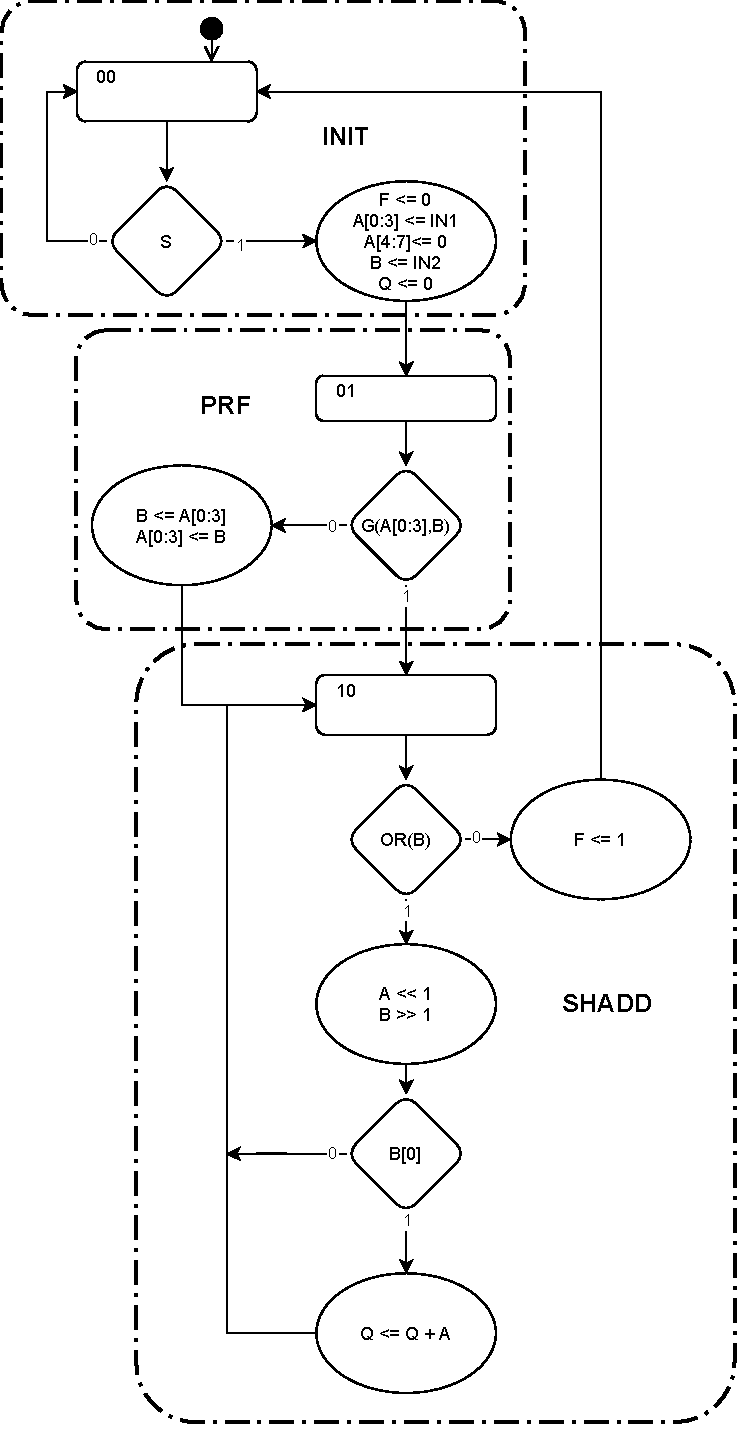
\includegraphics[scale=0.5]{./graphics/asmv1}
	\caption{نسخه ابتدایی طراحی شده}
	\label{fig:asmv1}
\end{figure}


اما در زمان سنتز اولیه این چارت به مشکلی برخوردیم و آن نبود تراشه‌های مناسب مالتیپلکسر \lr{TTL} بود که زمانی که چند مورد ورودی برای یک شیفت رجیستر داشتیم باید از آنها استفاده می‌کردیم. به همین دلیل بلوک پرفورمنس را از چارت خارج کردیم تا چارت نهایی به شکل \ref{fig:asmv2} دربیاید (توضیحات همان است فقط بلوک کارایی حذف شده است و استیت‌ها به دو کاهش یافته است).

\begin{figure}
	\centering
	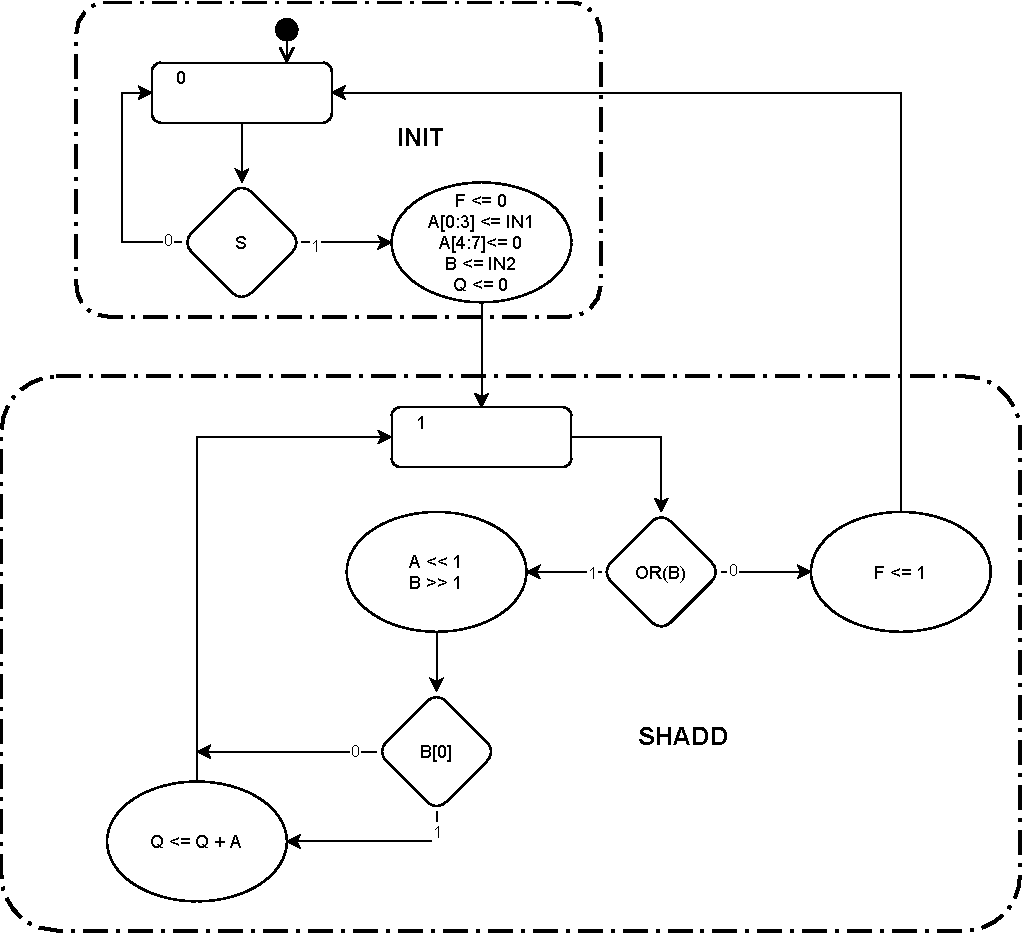
\includegraphics[scale=0.5]{./graphics/asmv2}
	\caption{نسخه اصلاح شده}
	\label{fig:asmv2}
\end{figure}

\subsection{سنتز و ساخت مدار}
در این مرحله به سنتز و ساخت مدار می‌پردازیم. در ابتدای کار مدار اصلی را طبق چارت طراحی شده پیاده‌سازی می‌کنیم. مدار از دو بخش اصلی \lr{Data Path (DP)} و \lr{Control Unit (CU)} تشکیل شده است که خطوط اصلی مدار در قسمت \lr{DP} تشکیل شده و اجزای نگه‌دارنده داده و انتقال دهنده آنها در این بخش وجود دارد. خطوط کنترل این خطوط و کنترل وضعیت مدار در بخش \lr{CU} وجود دارد. سیگنال‌های کنترلی از بخش کنترل به بخش مسیرداده می‌روند.

در ادامه ابتدا تراشه‌هایی که مورد استفاده قرار گرفته است بررسی می‌شوند و سپس بخش‌های مختلف مدار بررسی می‌شوند.

\subsubsection{تراشه‌هایی که مورد استفاده قرار گرفته است}
\label{chips}
\begin{itemize}
\item[\lr{74283}]
این تراشه یک جمع کننده چهار بیتی است که برای ساخت یک جمع کننده هشت بیتی از دوتای آن استفاده کرده‌ایم و به صورت آبشاری به هم متصل کرده ایم. نامگذاری پایه‌ها به صورت رایج انجام شده بود و نیازی به خواندن دیتاشیت نبود.

\item[\lr{74194}]
این یک شیفت رجیستر چهاربیتی است که چهار عمل برای آن در نظر گرفته شده است: بدون‌عمل، شیفت به راست، شیفت به چپ و بارگزاری داده. دارای یک ریست آسنکرون است. و بیتی که ورودی شیفت در آن قابل تعیین است (که ما بیت صفر را اضافه می‌کنیم). اعمال آن با توجه به خط سلکت آن به این شرح است:

\begin{latin}
$S_1 S_0$\\
00 $\rightarrow$ NOP\\
01 $\rightarrow$ Left \\
10 $\rightarrow$ Right\\
11 $\rightarrow$ Load 
\end{latin}
\item[\lr{74198}]
این یک شیفت رجیستر هشت بیتی با رفتار کاملا شبیه با تراشه 74194 است.

\item[\lr{2732}] این تراشه یک \lr{EPROM}
است و از آن برای دیکود کردن سون سگمنت‌هایی که برای نمایش نتیجه می‌خواستیم استفاده شده است. فایل‌های مربوط به داده شده به آن را به صورت دستی تهیه کرده ایم و به این صورت که هر کدام برای دو سون سگمنت استفاده می‌شود. برای ۱۶ آدرس ابتدایی آن داده در نظر گرفته ایم.

\item[\lr{7404}] این تراشه یک شامل شش گیت \lr{NOT} است که در ساخت بخش‌هایی از مدار استفاده شده است. چون به صورت گیت منطقی در نرم‌افزار آمده بود نیازی به مطالعه دیتاشیت نبود.

\item[\lr{7408}] این تراشه یک شامل چهار گیت \lr{AND} است که در ساخت بخش‌هایی از مدار استفاده شده است. چون به صورت گیت منطقی در نرم‌افزار آمده بود نیازی به مطالعه دیتاشیت نبود.

\item[\lr{7432}]  این تراشه یک شامل چهار گیت \lr{OR} است که در ساخت بخش‌هایی از مدار استفاده شده است. چون به صورت گیت منطقی در نرم‌افزار آمده بود نیازی به مطالعه دیتاشیت نبود.

\item[\lr{7474}]  این تراشه یک شامل دو فلیپ‌فلاپ نوع  \lr{D} است که در ساخت بخش‌هایی از مدار استفاده شده است. چون به صورت فلیپ‌فلاپ تک و با نام‌گذاری رایج در نرم‌افزار آمده بود نیازی به مطالعه دیتاشیت نبود.
\end{itemize}

\subsubsection{طراحی مسیرداده}
در این بخش باید داده‌ها و روابط بین آنها را که در دسیژن‌باکس‌ها آمده است را بیاوریم. با توجه به شکل \ref{fig:asmv2} این بخش را سنتز می‌کنیم:

\begin{itemize}
\item[\lr{A}]
یک شیفت رجیستر ۸ بیتی که چهاربیت داده ورودی آن به عدد اول و چهاربیت پرارزشتر آن به عدد ثابت صفر (زمین) متصل است.
\item[\lr{B}]
یک شیفت رجیستر ۴ بیتی که داده ورودی آن به ورودی دوم متصل است. از خروجی آن برای تولید دو سیگنال کنترلی استفاده می‌کنیم.
\item[\lr{C}]
یک شیفت رجیستر ۸ بیتی که جواب نهایی را در خود نگه‌میدارد و ورودی آن هم خروجی جمع کننده هشت بیتی است.
\item
یک جمع کننده که همواره مقدار درون شیفت رجیستر \lr{A} و رجیستر \lr{C} را در خود نگه میدارد.

\end{itemize}

همچنین به سیگنال‌های وضعیت زیر نیز نیاز خواهیم داشت:

\begin{itemize}
\item[\lr{B0}]
این سیگنال بیت اول شیفت رجیستر دوم است.
\item[\lr{ORB}]
این سیگنال «یا» منطقی چهار بیت شیفت رجیستر دوم است.
\item[\lr{S}]
این سیگنال شروع کار است.
\end{itemize}

\subsubsection{طراحی واحد کنترل}
در این بخش باید سیگنال‌های کنترلی را برای مسیر داده تولید کنیم. همچنین از یک فلیپفلاپ نوع دی برای نگه‌داری وضعیت فعلی مدار استفاده می‌کنیم. هر شیفت رجیستر (تراشه‌های 741794/74198) نیاز به دو سیگنال انتخاب (تغییر بین کارایی‌ها طبق بخش \ref{chips}) و یک سیگنال ریست دارند. یک سیگنال برای ورودی و یک سیگنال برای ریست فلیپ‌فلاپ \lr{F} و همین‌ها را برای فلیپ‌فلاپی که حالت را نگه می‌دارد نیز نیاز خواهیم داشت. 

از آنجایی که شیفت و لود رجیسترهای \lr{A,B} با یکدیگر انجام می‌شود از یک سیگنال تولید کرده و از آن برای هردو (با تغییرات جزئی در نحوه فرستادن آنها) استفاده می‌کنیم ($Q$ نمایش دهنده خروجی فلیپ‌فلاپ استیت‌های ماست).

\begin{latin}
\noindent
loadAB $= \overline{Q} \times S$\\
shiftAB $= Q  \times OR(B)$\\
clearAB = $1$ (Never will be cleared)\\
clearC $= \overline{Q} \times S = $ loadAB\\
loadC $= Q  \times OR(B) \times B[0]$\\
shiftC $= 0$ (Never will be shifted)
\end{latin}

با استفاده از این روابط سیگنال‌های مربوط به رجیسترها را به دست می‌آوریم:
\begin{latin}
\noindent
$A_{S0} = loadAB + shiftAB ,A_{S1} = loadAB$\\
$B_{S0} = loadAB = A_{S1} ,B_{S1} = loadAB + shiftAB = A_{S0}$\\
$C_{S0} = loadC ,C_{S1} = loadC$\\
$C_{clear} = \overline{clearC}$
\end{latin}

برای سیگنال \lr{F} هم صفر شدن \lr{B} را در نظر می‌گیریم.

با یک نگاه به جدول حالت می‌توانیم بگوییم که
$Q_D = (Q+S)(\overline{Q}+OR(B))$
(دقت کنید که سیگنال ست در زمانی که میخواهیم ست رخ بدهد صفر میشود نه یک).

\subsection{پیاده‌سازی}

با توجه به اینکه مشخصات طراحی توضیح داده شده است در این بخش فقط تصاویر آنرا می‌آوریم (تصاویر در دو صفحه قبل آمده اند).

\begin{figure}
	\centering
	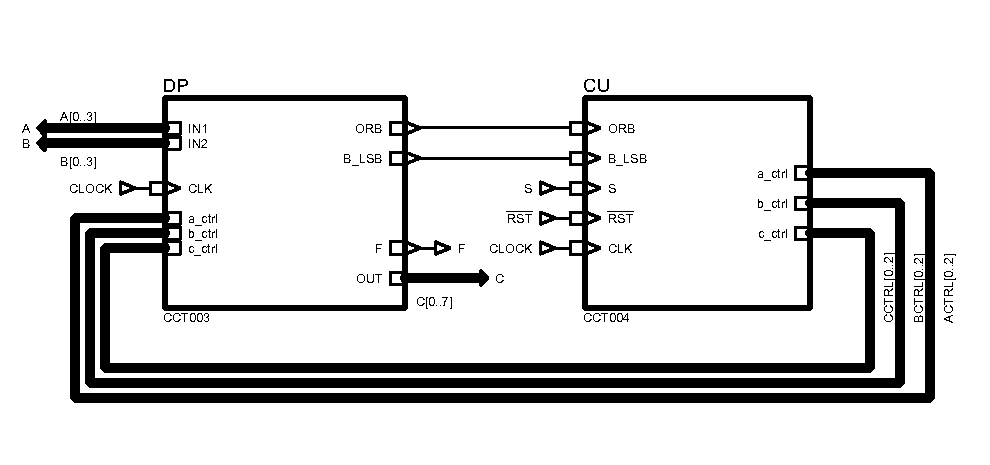
\includegraphics[scale=0.5]{./graphics/4bitmult}
	\caption{داخل ضرب کننده چهار بیتی}
\end{figure}


\begin{figure}
	\centering
	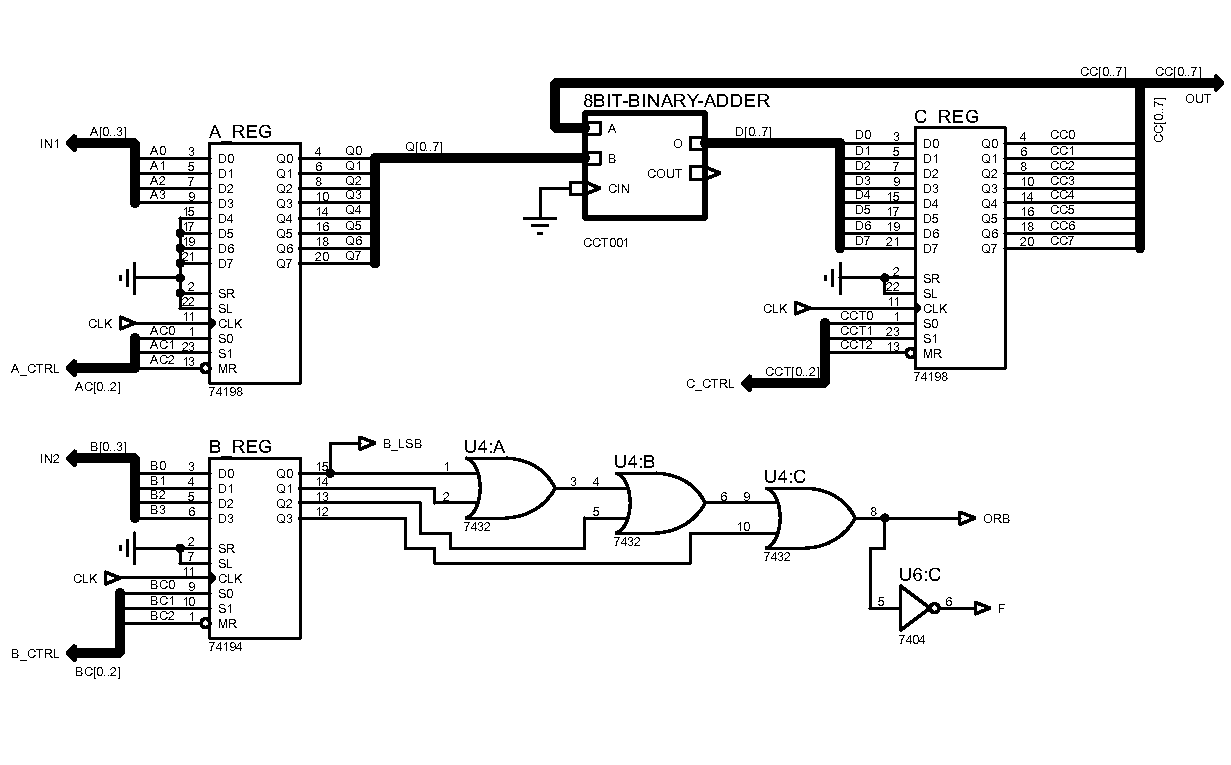
\includegraphics[scale=0.7]{./graphics/DP}
	\caption{مسیرداده}
\end{figure}


\begin{figure}
	\centering
	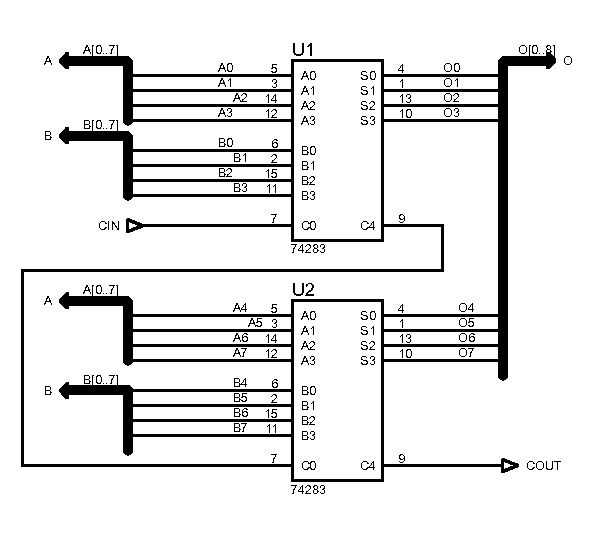
\includegraphics[scale=0.7]{./graphics/adder}
	\caption{جمع کننده استفاده شده در مسیرداده}
\end{figure}


\begin{figure}
	\centering
	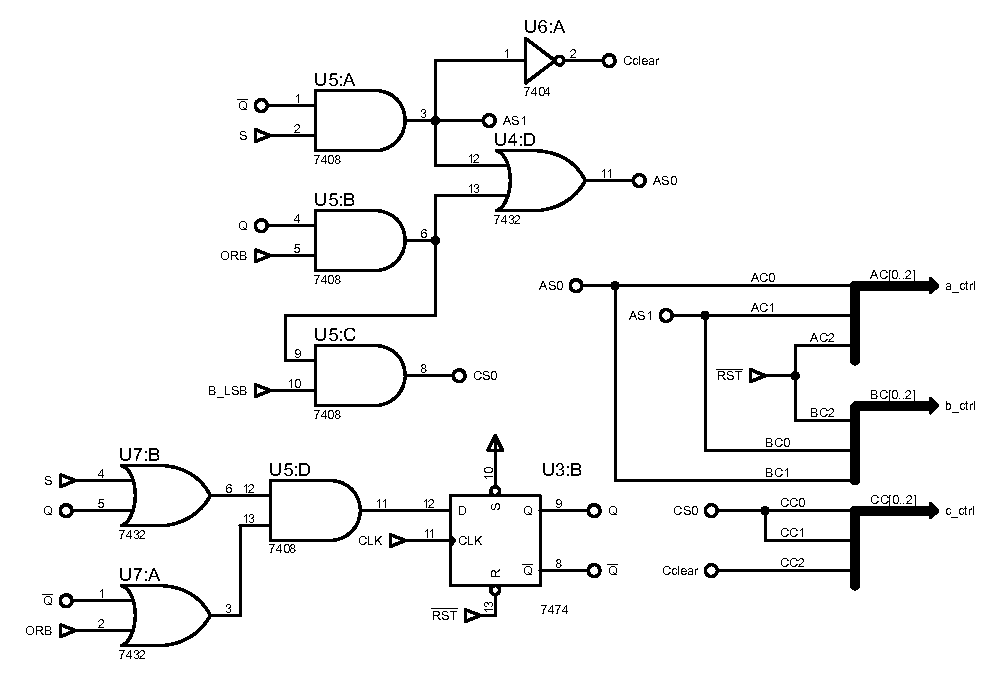
\includegraphics[scale=0.7]{./graphics/CU}
	\caption{واحد کنترل}
\end{figure}


\section{تست}
برای نمایش نتایج تست از \lr{7 Segments} استفاده شده است. برای اعداد ورودی قسمت غیراعشاری به صورت مستقیم متصل شده اند. قسمت اعشاری نیز به این صورت وصل شده اند که اگر کم ارزش ترین بیت روشن باشد 0/25 را خواهیم داشت و اگر بیت دوم روشن باشن 0.5 را خواهیم داشت که سیگنال مورد نیاز برای اینها تداخلی ندارد و می‌توان آنها را به صورت مستقیم به سون سگمنت‌ها متصل کرد.

برای نمایش خروجی‌ها از سه \lr{EPROM} استفاده کرده‌ایم که یک دیکودر هستند. دوتای آنها برای دیکود کردن ۴ بیت اعشار و دیگری برای دیکود کردن قسمت صحیح جواب است. داده نوشته شده در آنها در کنار فایل گزارش موجود است. هر کدام از آنها برای نمایش دو رقم دهدهی کافی هستند.

در ادامه چند تست انجام شده را مشاهده خواهید کرد که صحت آنها از نمایشگرها مشخص است:

\begin{figure}
	\centering
	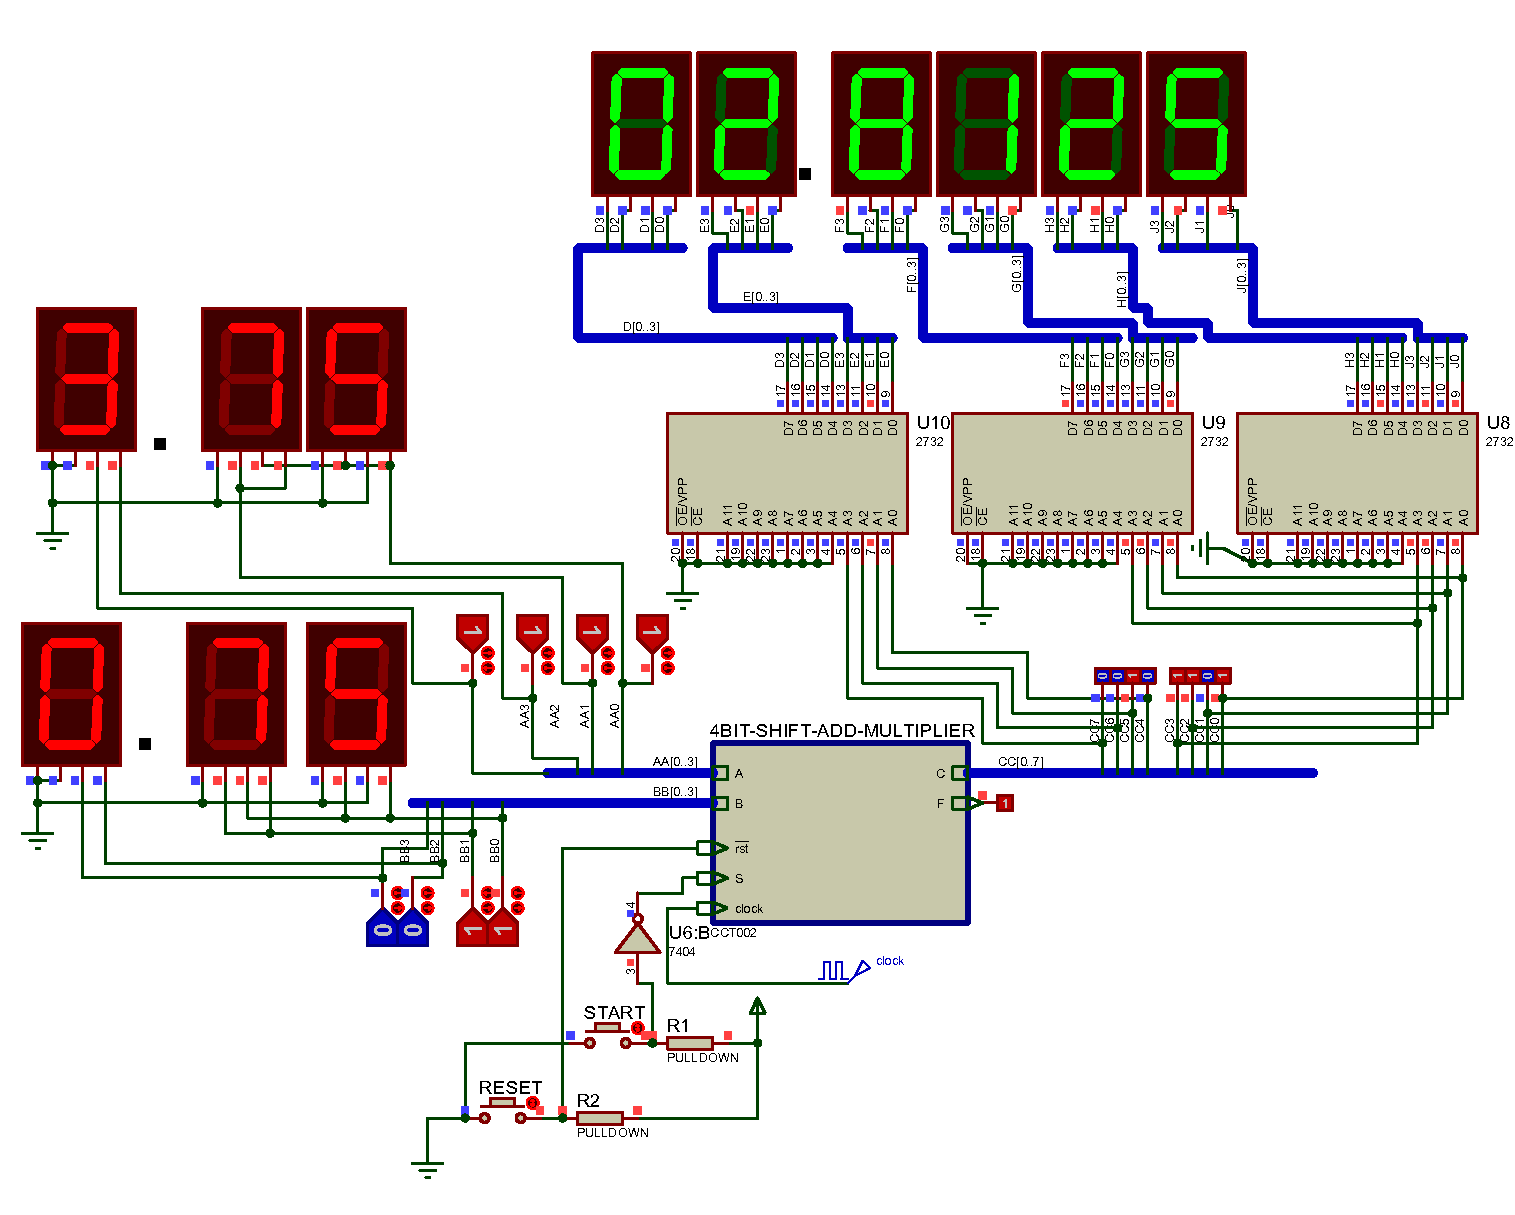
\includegraphics[scale=0.5]{./graphics/test1}
	\caption{تست ۱}
\end{figure}


\begin{figure}
	\centering
	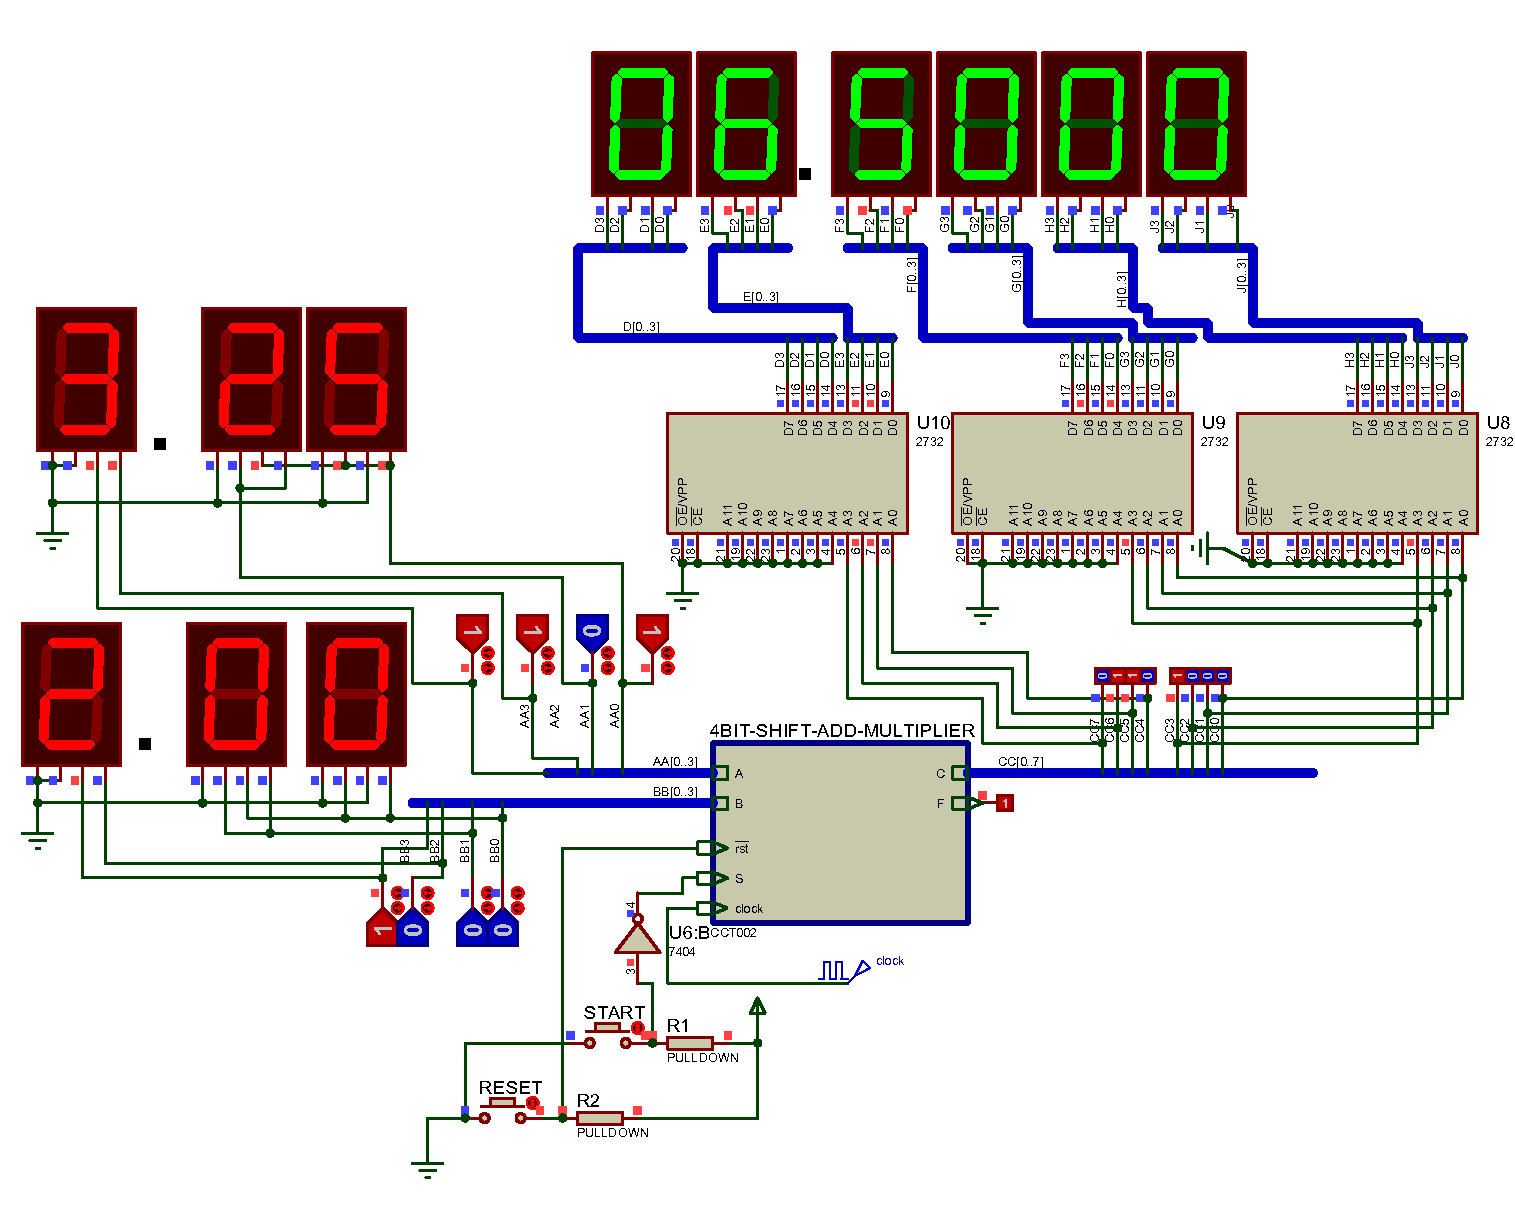
\includegraphics[scale=0.5]{./graphics/test2}
	\caption{تست ۲}
\end{figure}


\begin{figure}
	\centering
	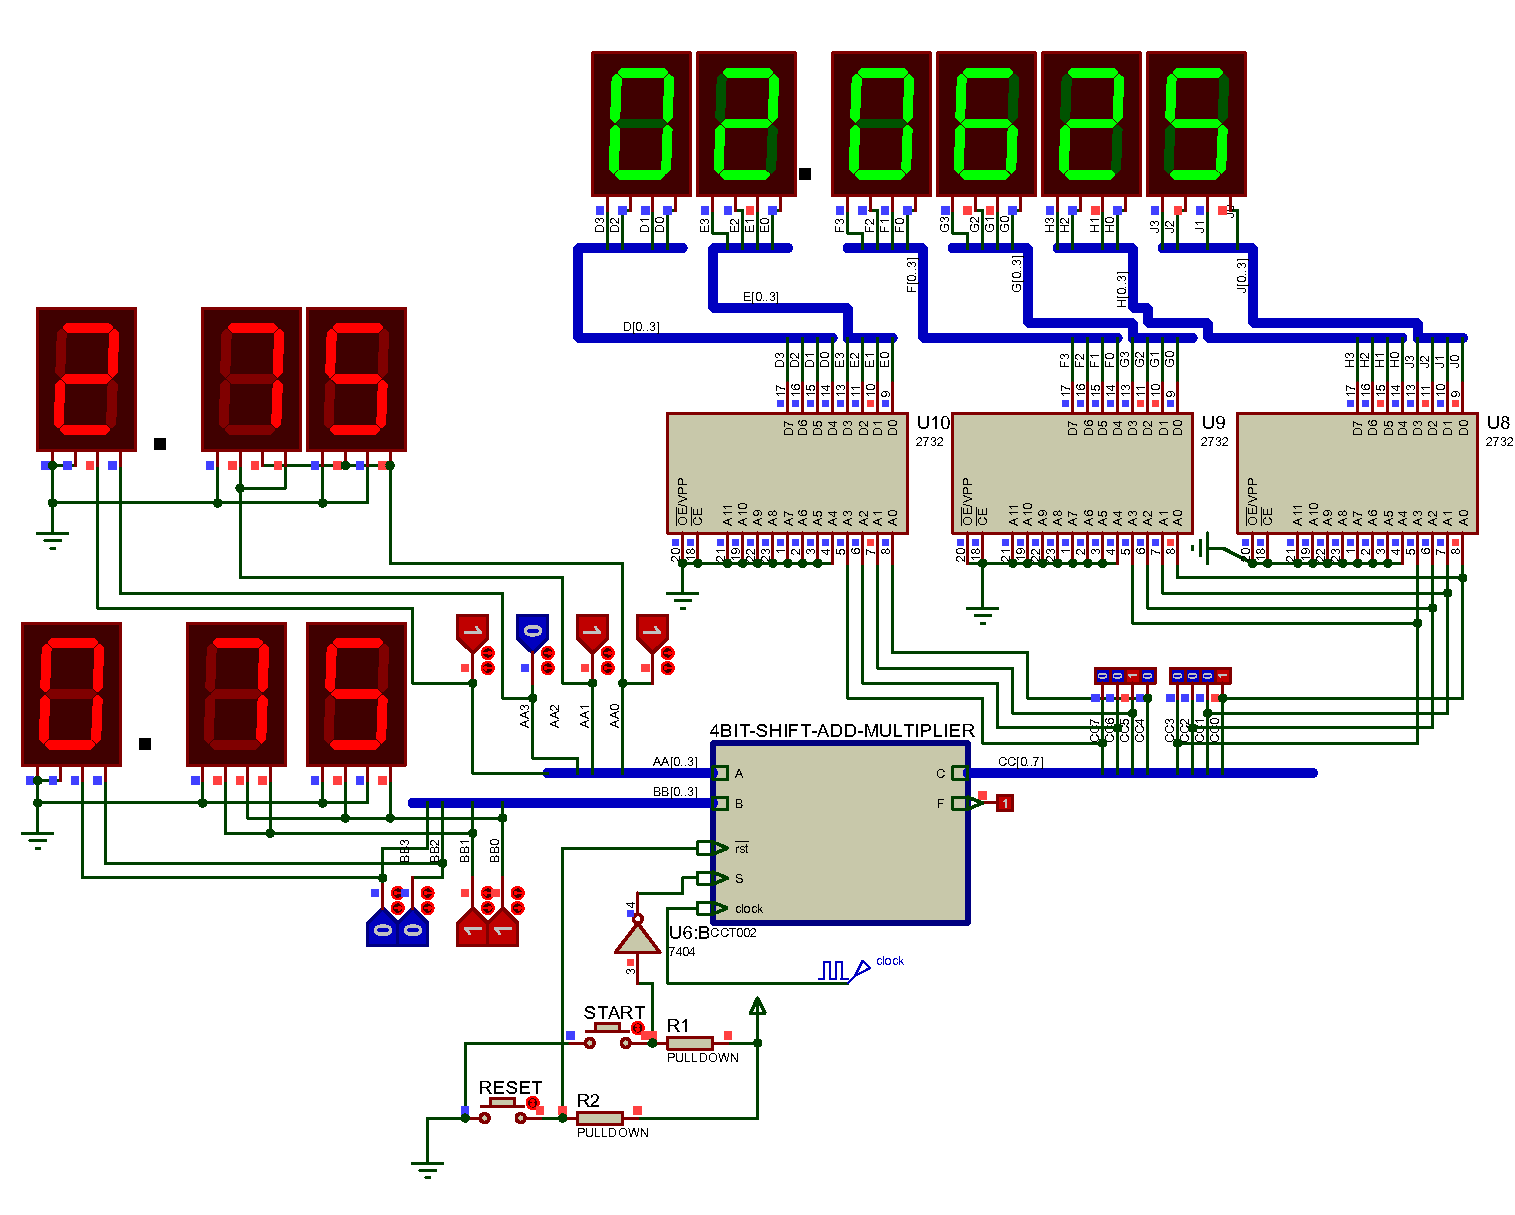
\includegraphics[scale=0.5]{./graphics/test3}
	\caption{تست ۳}
\end{figure}
\end{document}
 
